\chapter{Introduction}

The problem considered in this thesis arises from the Kronig-Penney model which describes an idealised quantum-mechanical system, that demonstrates a particle behaving as a matter wave moving in one-dimension trough an infinite periodic array of rectangular potential barriers, i.e. through a space area in which a potential attains a local maximum. Such an array commonly occurs in models of periodic crystal lattices where the potential is caused by ions in the crystal. They create an electromagnetic field around themselves and hence any particle moving through such a crystal would be subject to a periodic electromagnetic potential. Although a solid particle, simplified as a point mass, would be reflected at such a barrier, there is a possibility that the quantum particle, as it behaves like a wave, penetrates the barrier and continues its movement beyond\footnote{The likelihood that the particle will pass through the barrier is given by the transmission coefficient, whereas the likelihood that it is reflected is given by the reflection coefficient. Schrödinger's wave-equation allows these coefficients to be calculated.}. Assuming the spacing between all ions is $a$, the potential function $V(x)$ in the lattice can be approximated by a rectangular potential like this: % todo Martin remove footnote?

\begin{figure*}[h!] \centering
	  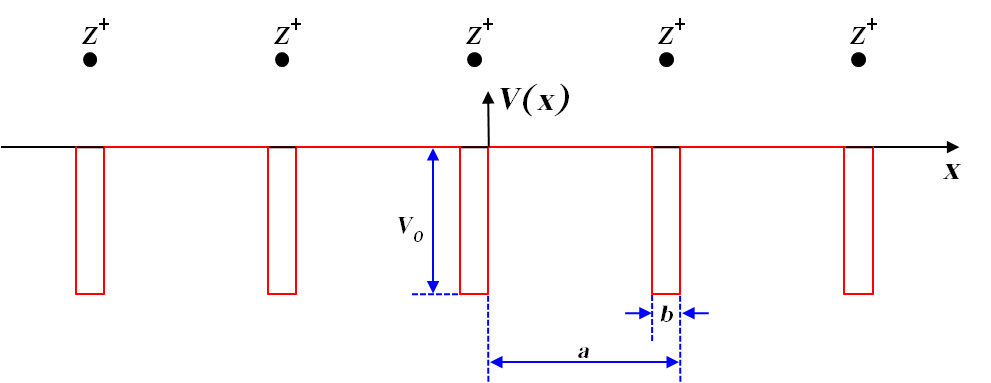
\includegraphics[width=0.7\textwidth]{Periodic_square_potential_130707} % todo Martin replace image
\end{figure*}

where $b$ is the \enquote{support} and $\rho$ the magnitude of the potential.

This thesis will examine the spectrum of an operator describing a special case of the Kronig-Penney model, namely by taking the limit $b \rightarrow 0$ with a finite modulus of the potential which represents the ion creating a finite singular potential. 

\section*{Mathematical Basics}

For the upcoming analysis we need some basic concepts from functional analysis and spectral theory I want to briefly recapitulate

\subsection*{Topics I don't know if I'm supposed to introduce them:} 
\begin{itemize}
	\item Introducing: Fourier series
	\item Introducing weak derivates
	\item Introducing: weak formulation
	\item Proving: $C_{c}^{\infty}(\R)$ is dense in $H^{1}(\R)$
	\item Proving: $H^1(R)$ is dense in $L^2$
	\item Proving: compact embedding theorem
	\item Defining: symmetric and self-Adjoint operators 
\end{itemize}
~\newline
Let $C_{c}^{\infty}$ denote the linear space containing all smooth function $f \colon \R \rightarrow \R$ with compact support, i.e. for $f \in C_{c}^{\infty}$ there exists a compact interval $I \subseteq \R$ such that $f(x) = 0$ for all $x \notin I$. Together with the supremums norm $\| \cdot \|_{\infty}$ is $C_{c}^{\infty}$ a normed vector space.

\subsection*{Hilbert and Sobolev spaces}
A normed vector space $(X, \| \cdot \|)$ is called a pre-Hilbert space, if there exists a scalar product $\langle \cdot, \cdot, \rangle$ on $X \times X$ such that
	\[ \| x \| = \langle x, x \rangle^{\frac{1}{2}} \] 

Any pre-Hilbert space that is additionally also a complete space is called a Hilbert space.

The Sobolev space $H^{k}$ is defined to be the subset of functions $f$ in $L^{2}(\R)$ such that the function $f$ and its weak derivatives up to some order $k$ have a $finite L^{2}$ norm. A

Furthermore, the space $H^{k}$ admits an inner product, which is defined in terms of the $L^2$ inner product: 
	\[ \langle u , v \rangle_{H^{k}} = \sum_{i=0}^{k} \left\langle D^{i}u , D^{i} v \right\rangle_{L^{2}}. \] 
The space $H^{k}$ becomes a Hilbert space with this inner product.

\subsection*{Distributions}
	On $C_{0}^{\infty}$ a sequence $(f_{n})$ converges against $f \in C_{0}^{\infty}$ if the support of all members of the sequence is in a compact interval $I \subset \R$, i.e.
	$$ \supp (f_{n}) \subseteq I \quad \forall n \in \N, $$
	and on this interval $f_{n}$ and all its derivatives converge uniformly against $f$, i.e.
	\[ \| f_{n}^{(i)} - f^{(i)} \|_{\infty} \rightarrow 0 \quad \text{ for } n \rightarrow \infty \]
	for all $i \in \N_{0}$. One can proof that this concept of convergence generates a topology on $C_{0}^{\infty}$ and one usually denoted with $D(\R)$ the space $C_{0}^{\infty}$ equipped with this topology. As the space of distribution, $D'(\R)$ we now denote all linear functionals on $C_{0}^{\infty}$ that are continuous with respect to this topology.
~\\ ~\\ % todo Markus by $\delta_{x_{0}} \coloneqq f(x_{0})$
An important example for a distribution is the Dirac delta function $\delta_{x_{0}}$ where $x_{0} \in \R$. It is defined as the limit of a weakly converging sequence of functionals over normed symmetric around $x_{0}$ cumulative distribution functions $\delta_{\epsilon}$, whereas the support of those cumulative distributions converges to zero. It holds $\delta_{x_{0}} = \lim_{\epsilon \rightarrow 0} \delta_{\epsilon}$ in $D'(\R)$. An example for such a sequence is be % todo Andrii can I say it like that
	\[ \delta_{\epsilon}(x) = \frac{1}{\sqrt{2 \pi} \epsilon} e^{-\frac{x^{2}}{2 \epsilon^{2}}}. \]
Which implies the definition
	\[ \delta_{x_{0}}(f) \coloneqq \int_{-\infty}^{\infty} \delta_{x_{0}} f(x) dx \coloneqq \lim_{\epsilon \rightarrow 0} \int_{-\infty}^{\infty} \delta_{\epsilon}(x - x_{0}) f(x) dx. \]
Moreover, is easily seen that $\delta_{x_{0}}(f) = \lim_{\epsilon \rightarrow 0} \delta_{\epsilon}(f) = f(x_{0})$. % todo Markus formulation
\begin{proof}
	We have
	\[ \int_{-\infty}^{\infty} f(x) \delta_{\epsilon}(x-x_{0}) dx = \frac{1}{\sqrt{2\pi} \epsilon} \int_{-\infty}^{\infty} f(x) e^{-\frac{(x - x_{0})^{2}}{2 \epsilon^{2}}} dx. \] 
	The substitution $z \coloneqq \frac{x - x_{0}}{\sqrt{2} \epsilon}$ implies 
	\[ \frac{1}{\sqrt{2\pi} \epsilon} \int_{-\infty}^{\infty} f(x) e^{-\frac{(x - x_{0})^{2}}{2 \epsilon^{2}}} dx = \frac{1}{\sqrt{2\pi} \epsilon} \sqrt{2} \epsilon \int_{-\infty}^{\infty} f(\sqrt{2} \epsilon z + x_{0}) e^{-z^{2}} dx. \]
	Using the taylor series of $f$ in $x_{0}$ we obtain
	\[ f(x) = f(x_{0}) + \mathcal{O}(\epsilon), \]
	Hence:
	\[ \lim_{\epsilon \rightarrow 0} \frac{1}{\sqrt{\pi}} \int_{-\infty}^{\infty} (f(x_{0}) + \mathcal{O}(\epsilon)) e^{-z^{2}} dz = f(x_{0}) \frac{1}{\sqrt{\pi}} \int_{-\infty}^{\infty} e^{-z^{2}} dz = f(x_{0}), \]
	where we used the fact that $\int_{-\infty}^{\infty} e^{-z^{2}}$ is a Gaussian integral and equal to $\sqrt{\pi}$. We can see that through :
	\[ \left( \int_{-\infty}^{\infty} e^{-x^{2}} dx \right) \left( \int_{-\infty}^{\infty} e^{-y^{2}} dy \right) = \int_{\R^{2}} e^{(x^{2} + y^{2})} d(x, y). \] 
	As we integrate over the whole $\R^{2}$ substituting in polar coordinates with the substition $z \coloneqq \rho^{2}$ yields
	\[ \int_{0}^{2 \pi} \int_{0}^{\infty} e^{-\rho^{2}} \rho d\rho d\varphi = 2 \pi \int_{0}^{\infty} e^{-\rho^{2}} \rho d\rho = \pi \int_{0}^{\infty} e^{-z^{2}} dz = \pi \left[ -e^{-z} \right]_{0}^{\infty} = \pi \]
\end{proof} 


\subsection*{Spektrum and resolvent of an operator}

Let $X$ be a Banach space and let $A \colon \mathcal{D} \rightarrow X$ be a  linear operator with domain $D(A) \supset X$. Let $I$ denote the identity operator on $X$. Then we define for any $\lambda \in \C$
	\begin{enumerate}[label=\alph*\upshape)]
		\item $\lambda$ belongs in the resolvent set of $A$, $\lambda \in \rho(A)$, if and only if
			\[ \lambda I - A \colon D(A) \rightarrow X \text{ bijective, i.e. } (\lambda I - A)^{-1} \colon X \rightarrow D(A) \text{ is a bounded linear operator.} \]
		\item $\sigma(A) = \C \setminus \rho(A)$ is called spectrum of $A$.
		\item $\lambda \in \rho(A) \rightarrow R(\lambda, A) = (\lambda - A)^{-1}$ is the resolvent function of $A$.
	\end{enumerate}	
	
\begin{theorem}
	The resolvent set $\rho(A) \subseteq \mathbb{C}$ of a bounded linear operator $A$ is an open set.
	
	\begin{proof}
		First, we note that the resolvent set is bounded as for $|\lambda| > \|A\|$ then $\| \lambda^{-1} A \| < 1$ and the operator $A - \lambda I = -\lambda (I - \lambda^{-1} A)$ has by the Neumann series the inverse
		$$ R(\lambda, A) = (A - \lambda I)^{-1} = - \sum_{k=0}^{\infty} \lambda^{-k-1} A^{k}. $$
		Now, to show that $\rho(A)$ is open we have proceed by showing that for any $\lambda \in \rho(A)$ there exist $\epsilon > 0$ such that all $\mu$ with $|\lambda- \mu| < \epsilon$ are also in $\rho(A)$. For that consider
		\begin{align*}
			A - \mu I & = A - \lambda I + (\lambda - \mu) I \\
					  & = (A - \lambda I)\left(I + (\lambda - \mu) (A - \lambda I)^{-1} \right).
		\end{align*}
		The last expression is an invertible operator because $T - \lambda I$ is invertible by the assumption and $I + (\lambda - \mu)(T - \lambda I)^{-1}$ is invertible again by the Neumann series, since $\|(\lambda - \mu)(A - \lambda I)^{-1}\| < 1$ if $\epsilon < \|(A - \lambda I)^{-1}\|$.
	\end{proof}
\end{theorem}